%%%%%%%%%%%%%%%%%%%%%%%%%%%%%%%%%%%%%%%%%
% baposter Landscape Poster
% LaTeX Template
% Version 1.0 (11/06/13)
%
% baposter Class Created by:
% Brian Amberg (baposter@brian-amberg.de)
%
% This template has been downloaded from:
% http://www.LaTeXTemplates.com
%
% License:
% CC BY-NC-SA 3.0 (http://creativecommons.org/licenses/by-nc-sa/3.0/)
%
%%%%%%%%%%%%%%%%%%%%%%%%%%%%%%%%%%%%%%%%%

%----------------------------------------------------------------------------------------
%	PACKAGES AND OTHER DOCUMENT CONFIGURATIONS
%----------------------------------------------------------------------------------------

\documentclass[landscape,a0paper,fontscale=0.324]{baposter} % Adjust the font scale/size here
% \documentclass[landscape,paperwidth=1978mm, paperheight=1183mm,fontscale=0.315]{baposter} % Adjust the font scale/size here


\usepackage{graphicx} % Required for including images
\graphicspath{{figures/}} % Directory in which figures are stored
\usepackage{wrapfig, lipsum} % wrap text round figure

\usepackage{calc}

\usepackage{hyperref} % \url, \href, etc ....

\usepackage{amsmath} % For typesetting math
\usepackage{amssymb} % Adds new symbols to be used in math mode

\usepackage{booktabs} % Top and bottom rules for tables
\usepackage{enumitem} % Used to reduce itemize/enumerate spacing
\usepackage{palatino} % Use the Palatino font
\usepackage[font=small,labelfont=bf]{caption} % Required for specifying captions to tables and figures

\usepackage{multicol} % Required for multiple columns
\setlength{\columnsep}{1.5em} % Slightly increase the space between columns
\setlength{\columnseprule}{0mm} % No horizontal rule between columns


\usepackage{tikz} % Required for flow chart
\usetikzlibrary{shapes,arrows} % Tikz libraries required for the flow chart in the template

\newcommand{\compresslist}{ % Define a command to reduce spacing within itemize/enumerate environments, this is used right after \begin{itemize} or \begin{enumerate}
\setlength{\itemsep}{0.5pt}
\setlength{\parskip}{0pt}
\setlength{\parsep}{0pt}
}

\definecolor{lightblue}{rgb}{0.145,0.6666,1} % Defines the color used for content box headers
\definecolor{alizarin}{rgb}{0.82, 0.1, 0.26}
\definecolor{applegreen}{rgb}{0.55, 0.71, 0.0}
\definecolor{auburn}{rgb}{0.43, 0.21, 0.1}
\definecolor{candyapplered}{rgb}{1.0, 0.03, 0.0}
\definecolor{charcoal}{rgb}{0.21, 0.27, 0.31}
\definecolor{coolblack}{rgb}{0.0, 0.18, 0.39}
\definecolor{babyblue}{rgb}{0.54, 0.81, 0.94}


\begin{document}

\begin{poster}
{
headerborder=closed, % Adds a border around the header of content boxes
colspacing=1em, % Column spacing
bgColorOne=white, % Background color for the gradient on the left side of the poster
bgColorTwo=white, % Background color for the gradient on the right side of the poster
borderColor=babyblue, % Border color
headerColorOne=black, % Background color for the header in the content boxes (left side)
headerColorTwo=babyblue, % Background color for the header in the content boxes (right side)
headerFontColor=white, % Text color for the header text in the content boxes
boxColorOne=white, % Background color of the content boxes
textborder=roundedleft, % Format of the border around content boxes, can be: none, bars, coils, triangles, rectangle, rounded, roundedsmall, roundedright or faded
eyecatcher=true, % Set to false for ignoring the left logo in the title and move the title left
headerheight=0.16\textheight, % Height of the header
headershape=roundedright, % Specify the rounded corner in the content box headers, can be: rectangle, small-rounded, roundedright, roundedleft or rounded
headerfont=\Large\bf\textsc, % Large, bold and sans serif font in the headers of content boxes
%textfont={\setlength{\parindent}{1.5em}}, % Uncomment for paragraph indentation
linewidth=0.75pt % Width of the border lines around content boxes
}
%----------------------------------------------------------------------------------------
%	TITLE SECTION 
%----------------------------------------------------------------------------------------
%
{
\includegraphics[height=6.5em]{../../logos/ntua.png} 
\includegraphics[height=6.5em]{../../logos/noa1.png}} % First university/lab logo on the left
% {\par{\textsc{European Geosciences Union General Assembly 2019 Vienna | Austria | 7 - 12 April 2015}}}
{\bf\textsc{Tectonic Strain Distribution over Europe from EPN data}\vspace{0.3em} } % Poster title
{\large Dimitris Anastasiou \textsuperscript{1,2}, Athanassios Ganas \textsuperscript{2}, Julliet Legrand \textsuperscript{3}, Carine Bruyninx \textsuperscript{3}, Xanthos Papanikolaou \textsuperscript{1,2}, Varvara Tsironi \textsuperscript{2}, Vasilis Kapetanidis \textsuperscript{4} 
{\small \par{\textsuperscript{1} National Technical University of Athens, Dionysos Satellite Observatory, Greece (danast@mail.ntua.gr) -- \textsuperscript{2} National Observatory of Athens, Institute of Geodynamics, Greece} 
\par{\textsuperscript{3} Royal Observatory of Belgium, Brussels, Belgium --  \textsuperscript{4} National ana Kapodistrian University of Athens, Department of Geology, Greece. }} \vspace{0.3em}
\par{\textsc{European Geosciences Union General Assembly 2019 Vienna | Austria | 7 - 12 April 2015}} 
\vskip 0.2cm
{
\includegraphics[height=2.5em]{../../logos/gein_logo.png} 
\includegraphics[height=2.5em]{../../logos/egu19_logo.png} 
\includegraphics[height=2.5em]{../../logos/epos_logo_big.jpg}} % Second university/lab logo on the right

 }
{
\includegraphics[height=6.5em]{../../logos/logo_orb.png} 
\includegraphics[height=6.5em]{../../logos/logo_uoa_blue.png}} % Second university/lab logo on the right
%----------------------------------------------------------------------------------------
%	INTRODUCTION
%----------------------------------------------------------------------------------------

\headerbox{Introduction}{name=introduction,column=0,row=0}{
\texttt{StrainTool} is a software package that enables the estimation and 
visualization of Strain Tensor parameters, given list of data points on the earth's 
crust along with their respective tectonic velocities. It consists of three basic
components:
\begin{itemize}
  \item a python package (library) \texttt{pystrain},
  \item a (main) program \texttt{StrainTensor.py} and
  \item a list of (shell) scripts to visualize results
\end{itemize}

\texttt{StrainTool} was developed in the framework of \emph{HELPOS}; it
is a free and open-source software project, distributed under the \emph{MIT License}.

A detailed introduction to \texttt{StrainTool}, a how-to guide, usage examples 
and discussion on the implemented methodologies is available on the web, at 
\texttt{https://dsolab.github.io/StrainTool/}.

% \vspace{0.3em} % When there are two boxes, some whitespace may need to be added if the one on the right has more content
}

%----------------------------------------------------------------------------------------
%	DATASET
%----------------------------------------------------------------------------------------

\headerbox{Velocity field - ETRF14}{name=data,column=2, span=2,row=0}{
% \vfill
\begin{minipage}[c]{0.24\linewidth}
  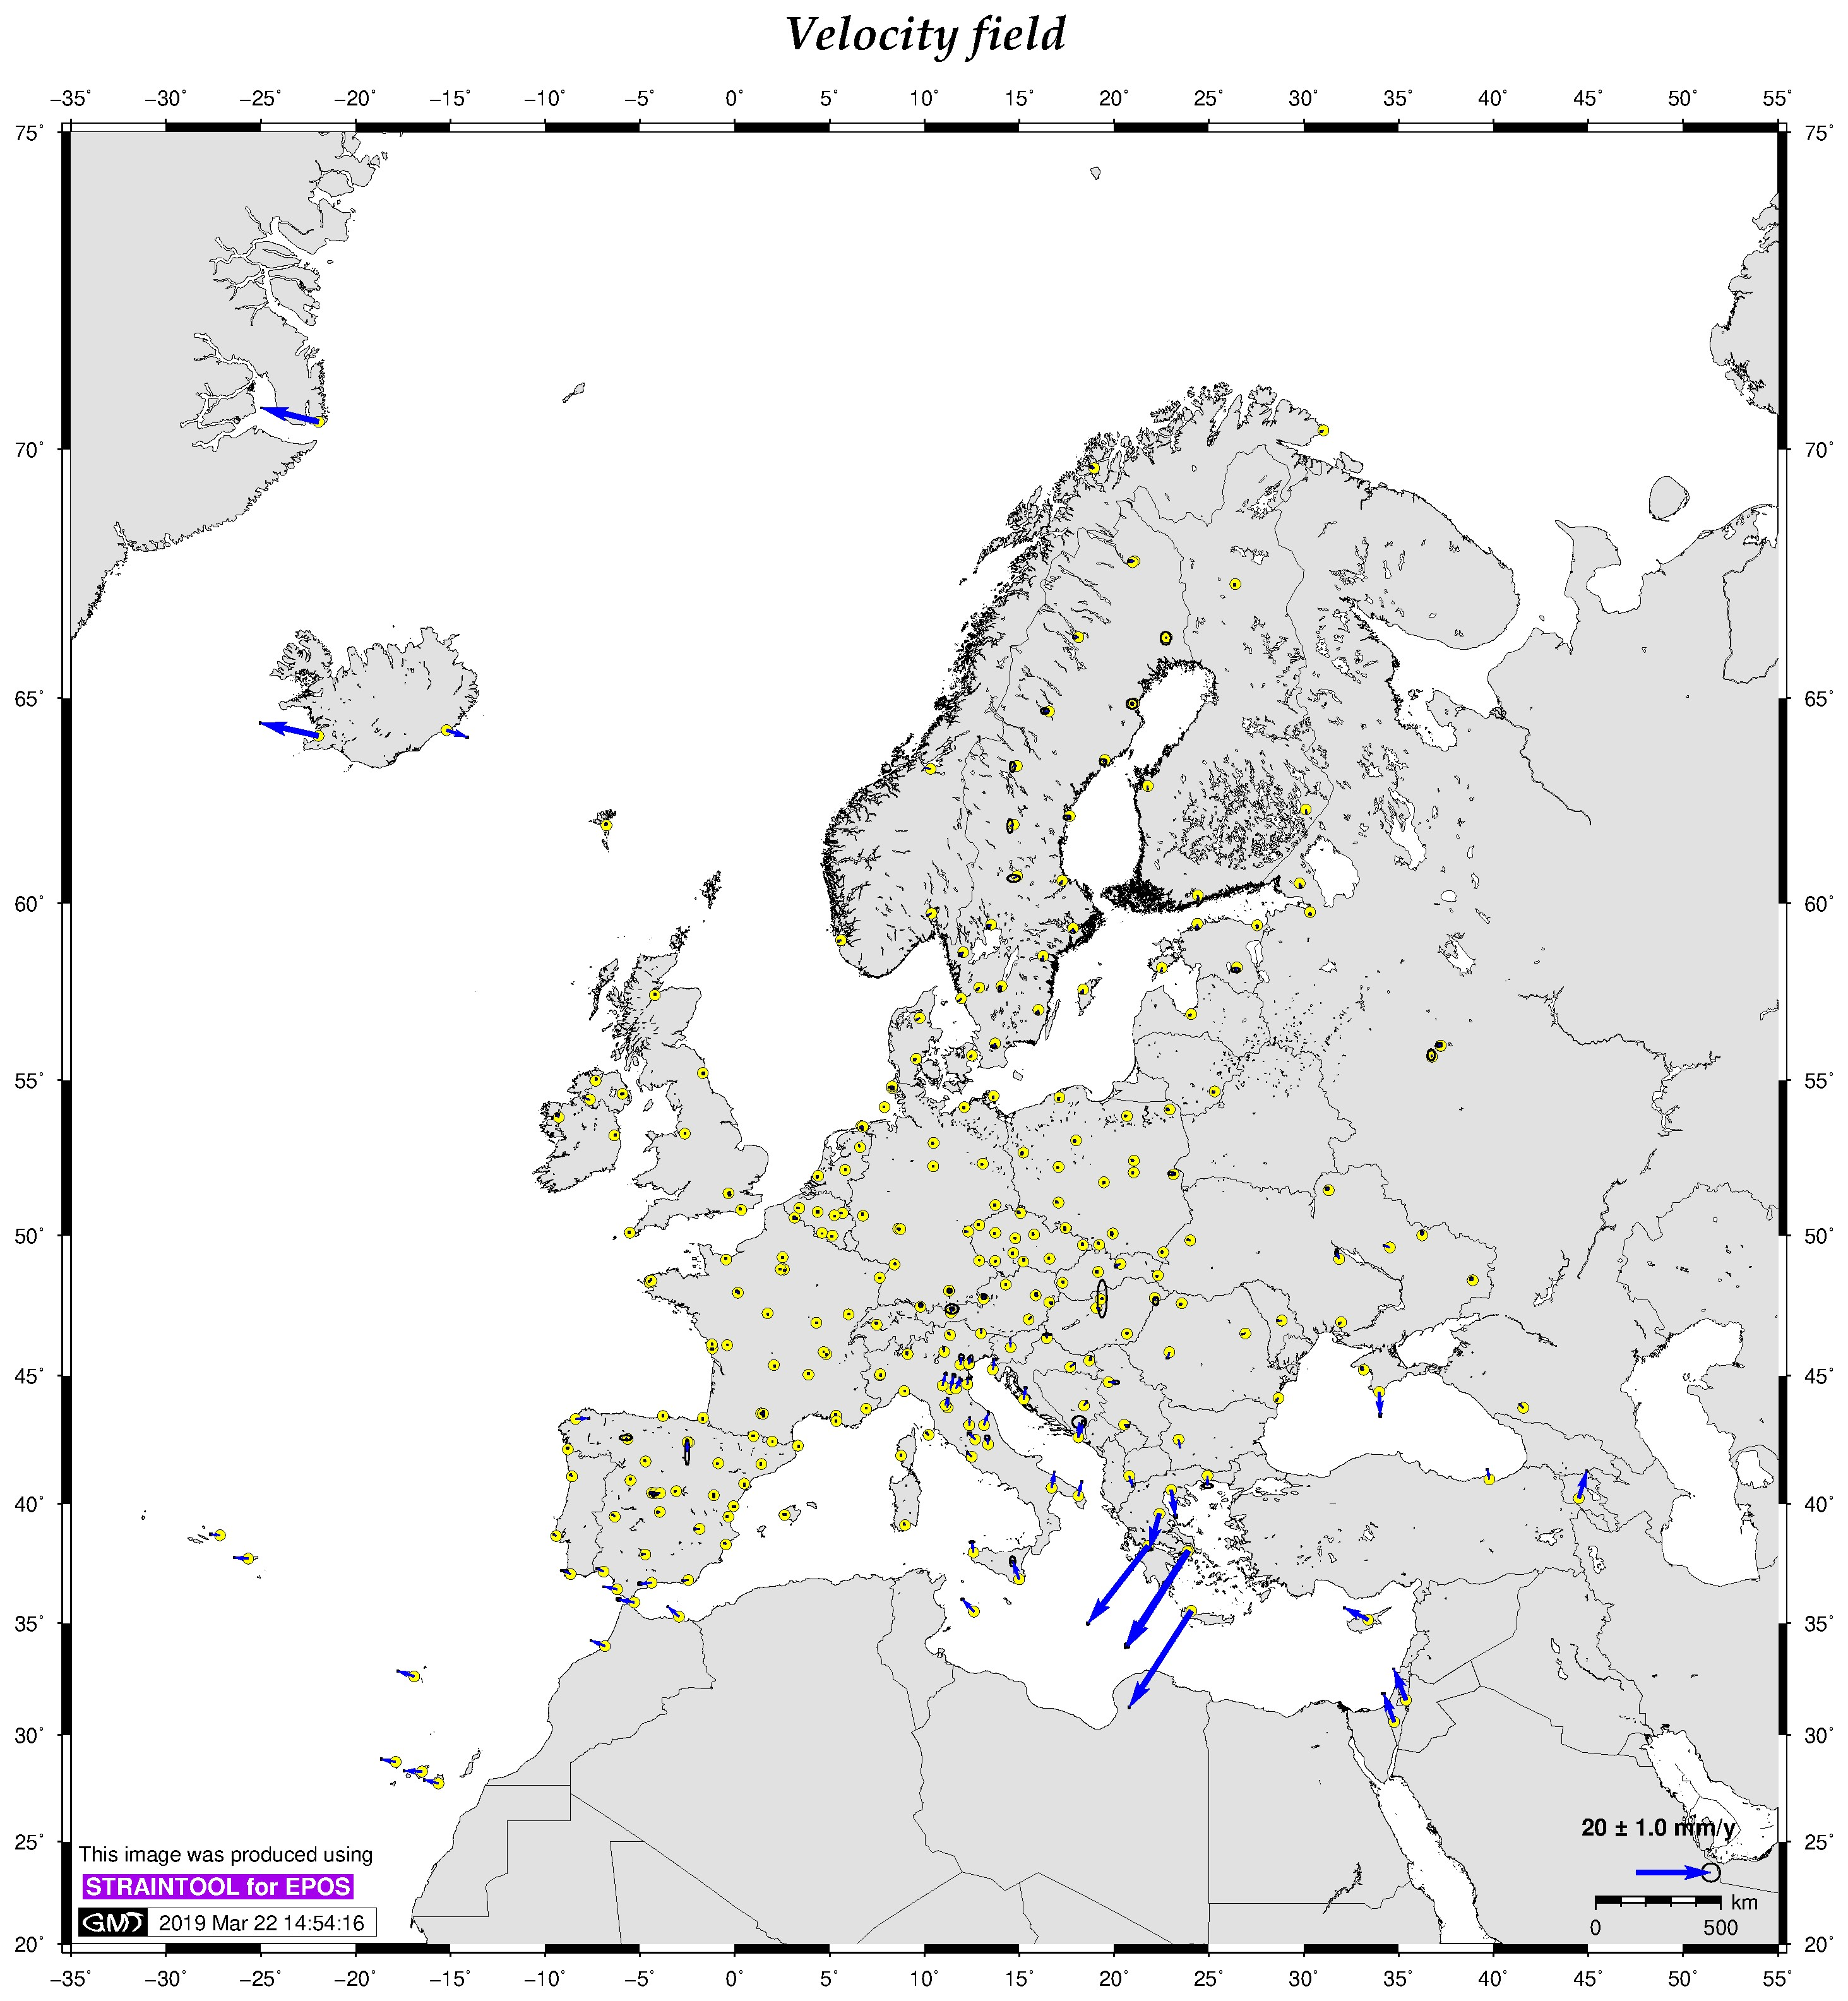
\includegraphics[height=13em]{vel_field.jpg}
\end{minipage}
\begin{minipage}[c]{0.74\linewidth}
A total number of 302 GNSS stations of EUREF Permanent Network (EPN) were selected on the base of the following criteria: 
a) station have observations time period longer than 3 years,
b) one velocity per station and
c) stations with largevelocity changes excluded.
The stations positions are computed with several geodetic software packages and then we used CATREF to estimate multi-year positions and velocity solution. The available dataset comprises the velocity field extracted from the C2010 EPN solution.

Reference frame of the velocity field is ETRF014 which is the realization of ETRS89 corresponding to ITRF14. According to EUREF Technical Report 1, the ETRS89 is fixed to the stable part of Eurasia tectonic plate. For the transformation from ITRF2014 to ETRF2014 the three translation components are set to zero and the rotational rates (Eurasia angular velocity components) are taken from \textbf{Altamimi et al. 2017}.
\end{minipage}


% \vspace{0.3em} % When there are two boxes, some whitespace may need to be added if the one on the right has more content
}

% %----------------------------------------------------------------------------------------
% %	RESULTS 1
% %----------------------------------------------------------------------------------------
% 
% \headerbox{Different Models Setup}{name=results,column=3,span=1,row=0}{
% 
% 
% }

%----------------------------------------------------------------------------------------
%	REFERENCES
%----------------------------------------------------------------------------------------

\headerbox{References}{name=references,column=0, span=2, above=bottom}{
\begin{minipage}[b]{0.92\linewidth}
{\scriptsize
\textbf{Altamimi Z.}, L. Métivier, P. Rebischung, H. Rouby, and X. Collilieux (2017) ITRF2014 plate motion model, Geophysical Journal International, Volume 209, Issue 3, 1 June 2017, Pages 1906-1912, https://doi.org/10.1093/gji/ggx136.

\textbf{Shen, Z.-K.}, M. Wang, Y. Zeng, and F. Wang, (2015), Strain determination using spatially discrete geodetic data, Bull. Seismol. Soc. Am., 105(4), 2117-2127, doi: 10.1785/0120140247

\textbf{Veis, G.}, Billiris, H., Nakos, B., and Paradissis, D. (1992), Tectonic strain in greece from geodetic measurements, C.R.Acad.Sci.Athens, 67:129--166

\textbf{Wessel, P.}, W. H. F. Smith, R. Scharroo, J. F. Luis, and F. Wobbe, Generic Mapping Tools: Improved version released, EOS Trans. AGU, 94, 409-410, 2013
}
\end{minipage}
\begin{minipage}[b]{0.06\linewidth}
%------------------------------------------
% \begin{wrapfigure}{c}{1.5cm}

\includegraphics[height=5em]{../../logos/graphic_egu_photo_yes.png}
% \caption{A wrapped figure going nicely inside the text.}\label{wrap-fig:1}
% \end{wrapfigure}
%------------------------------------------
\end{minipage}
}

%----------------------------------------------------------------------------------------
%	FUTURE RESEARCH
%----------------------------------------------------------------------------------------

\headerbox{Future Research}{name=futureresearch,column=2,aligned=references,above=bottom}{ 

We consider \texttt{StrainTool} to be a work-in-progress; we plan on augmenting its
functionality and provide further computation capabilities. Currentlly, we are 
working on a twofold approach: 
\begin{itemize} 
  \item first, enable the formulation of non-regular grids. 
  This will enable the construction of grids that are more dense in regions of high 
  data density and sparser at regions that lack data points.
  \item second, introduction of fault information. Faults can have a big impact
  in strain tensors parameters as their existance could cause discontinuities; the
  absence or mismodelling of such information, can result in non-realistic estimates.
\end{itemize}

Our aim is to keep the software user-friendly and efficient and hope for its 
adoption and wide usage within the scientific community.
}

%----------------------------------------------------------------------------------------
%	FUNDING
%----------------------------------------------------------------------------------------

\headerbox{FUNDING BY HELPOS}{name=funding,column=3,aligned=references,above=bottom}{ 

{\footnotesize We acknowledge support of this research by the project "HELPOS - Hellenic Plate Observing System" (MIS
5002697) which is implemented under the Action "Reinforcement of the Research and Innovation Infrastructure",
funded by the Operational Programme "Competitiveness, Entrepreneurship and Innovation" (NSRF 2014-2020).  
% and co-financed by Greece and the European Union.
}
}

%----------------------------------------------------------------------------------------
%	RESULTS 2
%----------------------------------------------------------------------------------------

\headerbox{Results and Discussion}{name=resval,column=2,span=2,row=0,below=data,above=references}{

\begin{minipage}[b]{0.62\linewidth}
Strain-rate results from 302 permanent European GNSS stations present in these maps. The vertical velocity component is ignored in this stage and other sources of deformation (GIA, hydrological, anthropogenic et al.) are not considered in the preliminary interpretation. Different model setups (variable grid-size, deistance from cell-center, smoothing parameters etc.) were used for estimation of strain rates. We present results estimated using the following model:

\begin{center}
\begin{tabular}{ c | c | c | c | c }
\hline
 grid-size & ltype & dmin & dmax & Wt \\ 
% \hline
  0.5$^{\circ} $x0.5$^{\circ} $ & gaussian & 1 km  & 500 km & 6 and 12   \\
\hline
 \end{tabular}
\end{center}

Overall, our first results reproduce the gross features of tectonic deformation in Southern Europe, such as NE-SW extension across the Apennines (Italy), NNW-SSE compression across the Alboran Sea (western Mediterranean) and N-S extension in mainland Greece. Large areas of central and Northern Europe show small strain rates (less than 10 ns/yr; 2nd invariant of the tensor).

% \begin{minipage}[t]{0.48\linewidth}
     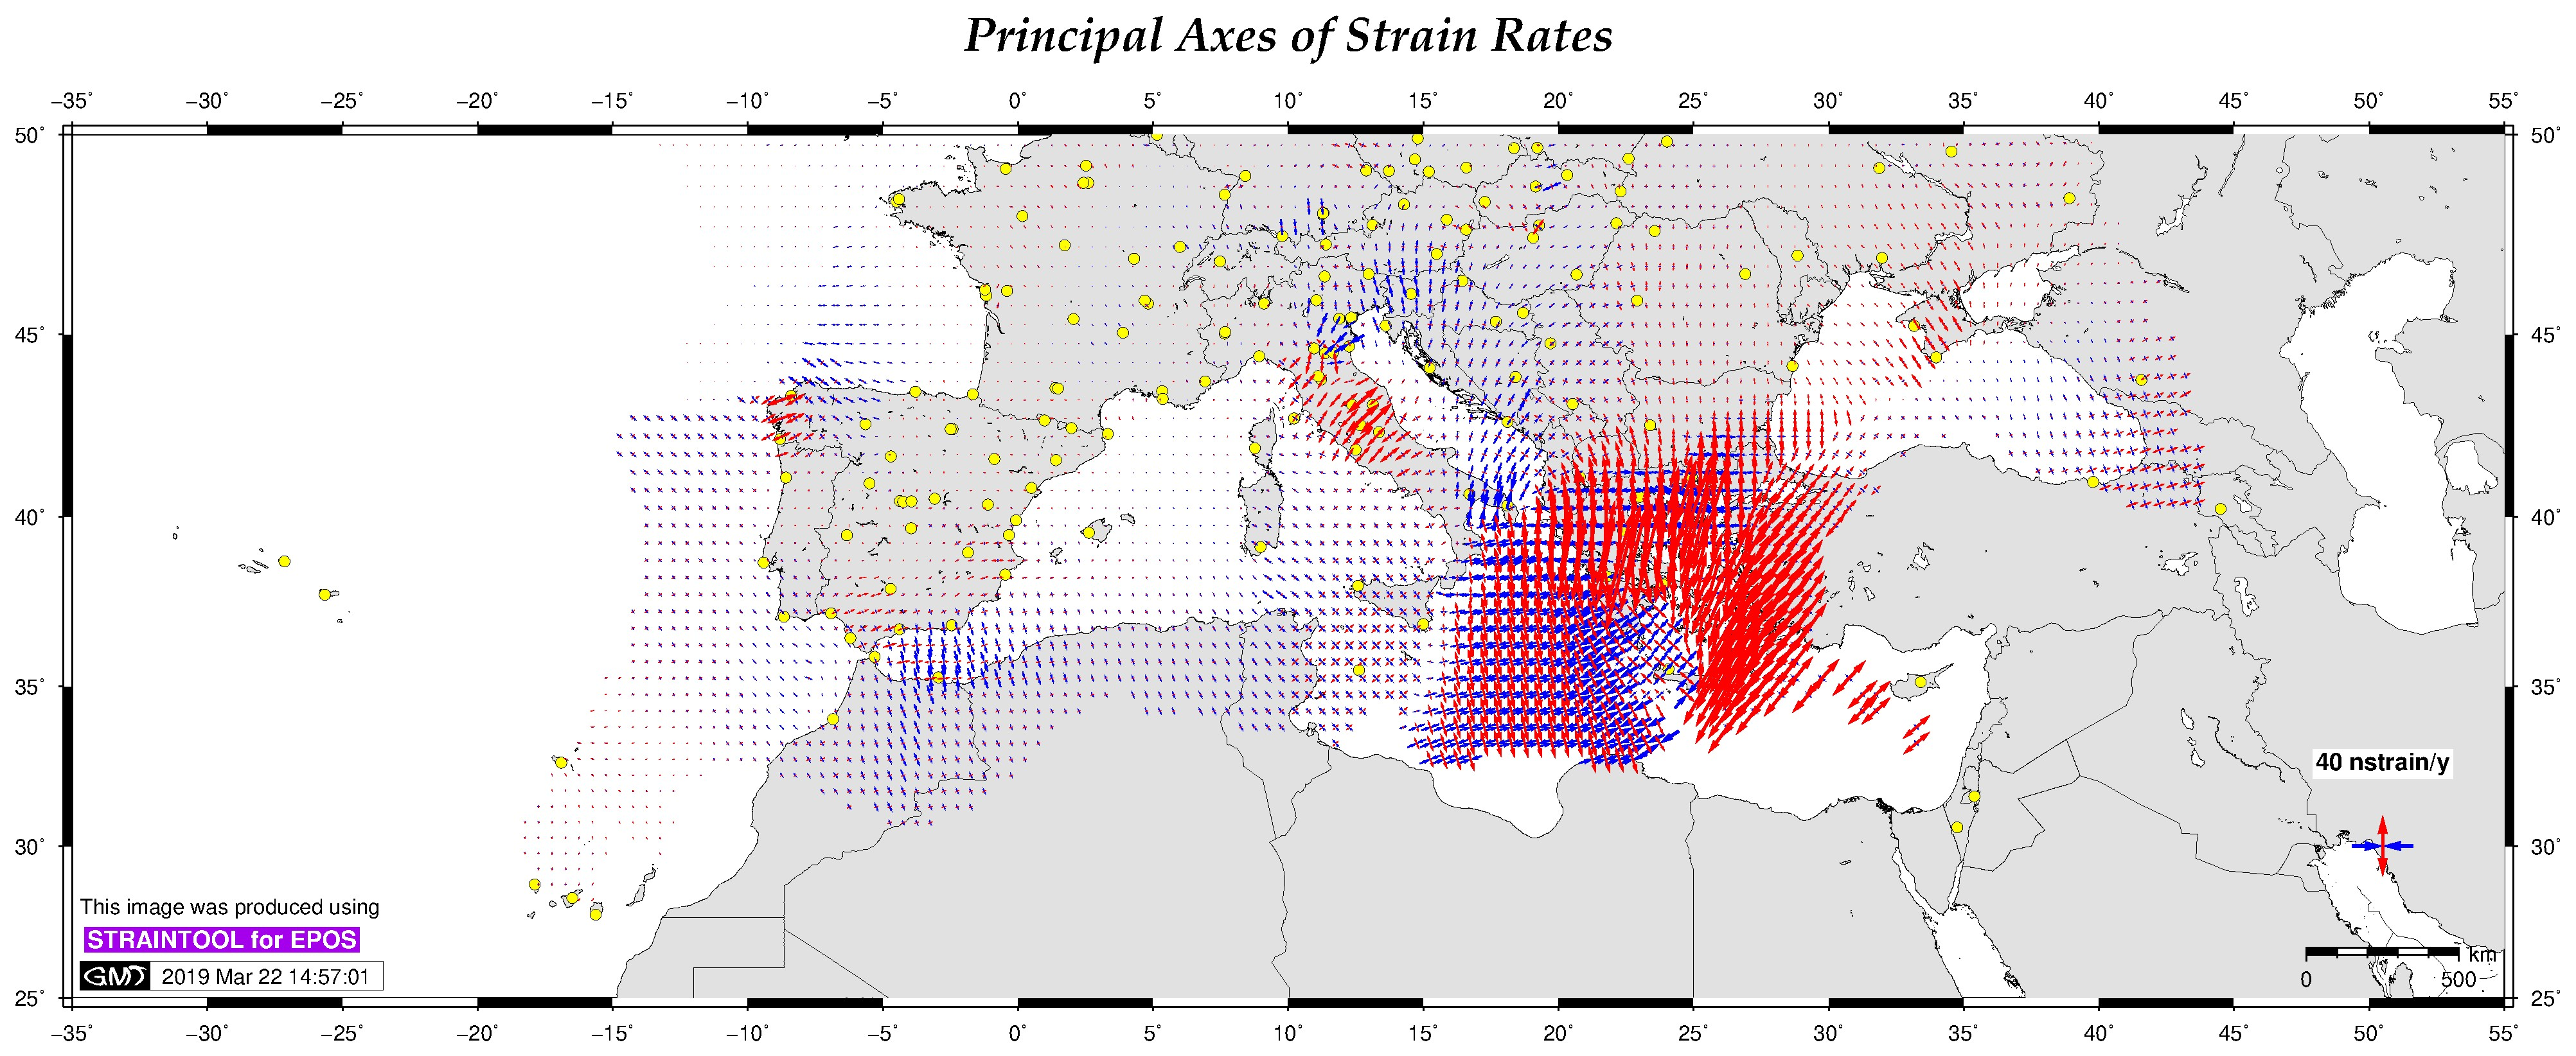
\includegraphics[width=\textwidth]{e14s050506-output_str-S.jpg}
% \end{minipage}\hfill
% \begin{minipage}[t]{0.48\linewidth}
%      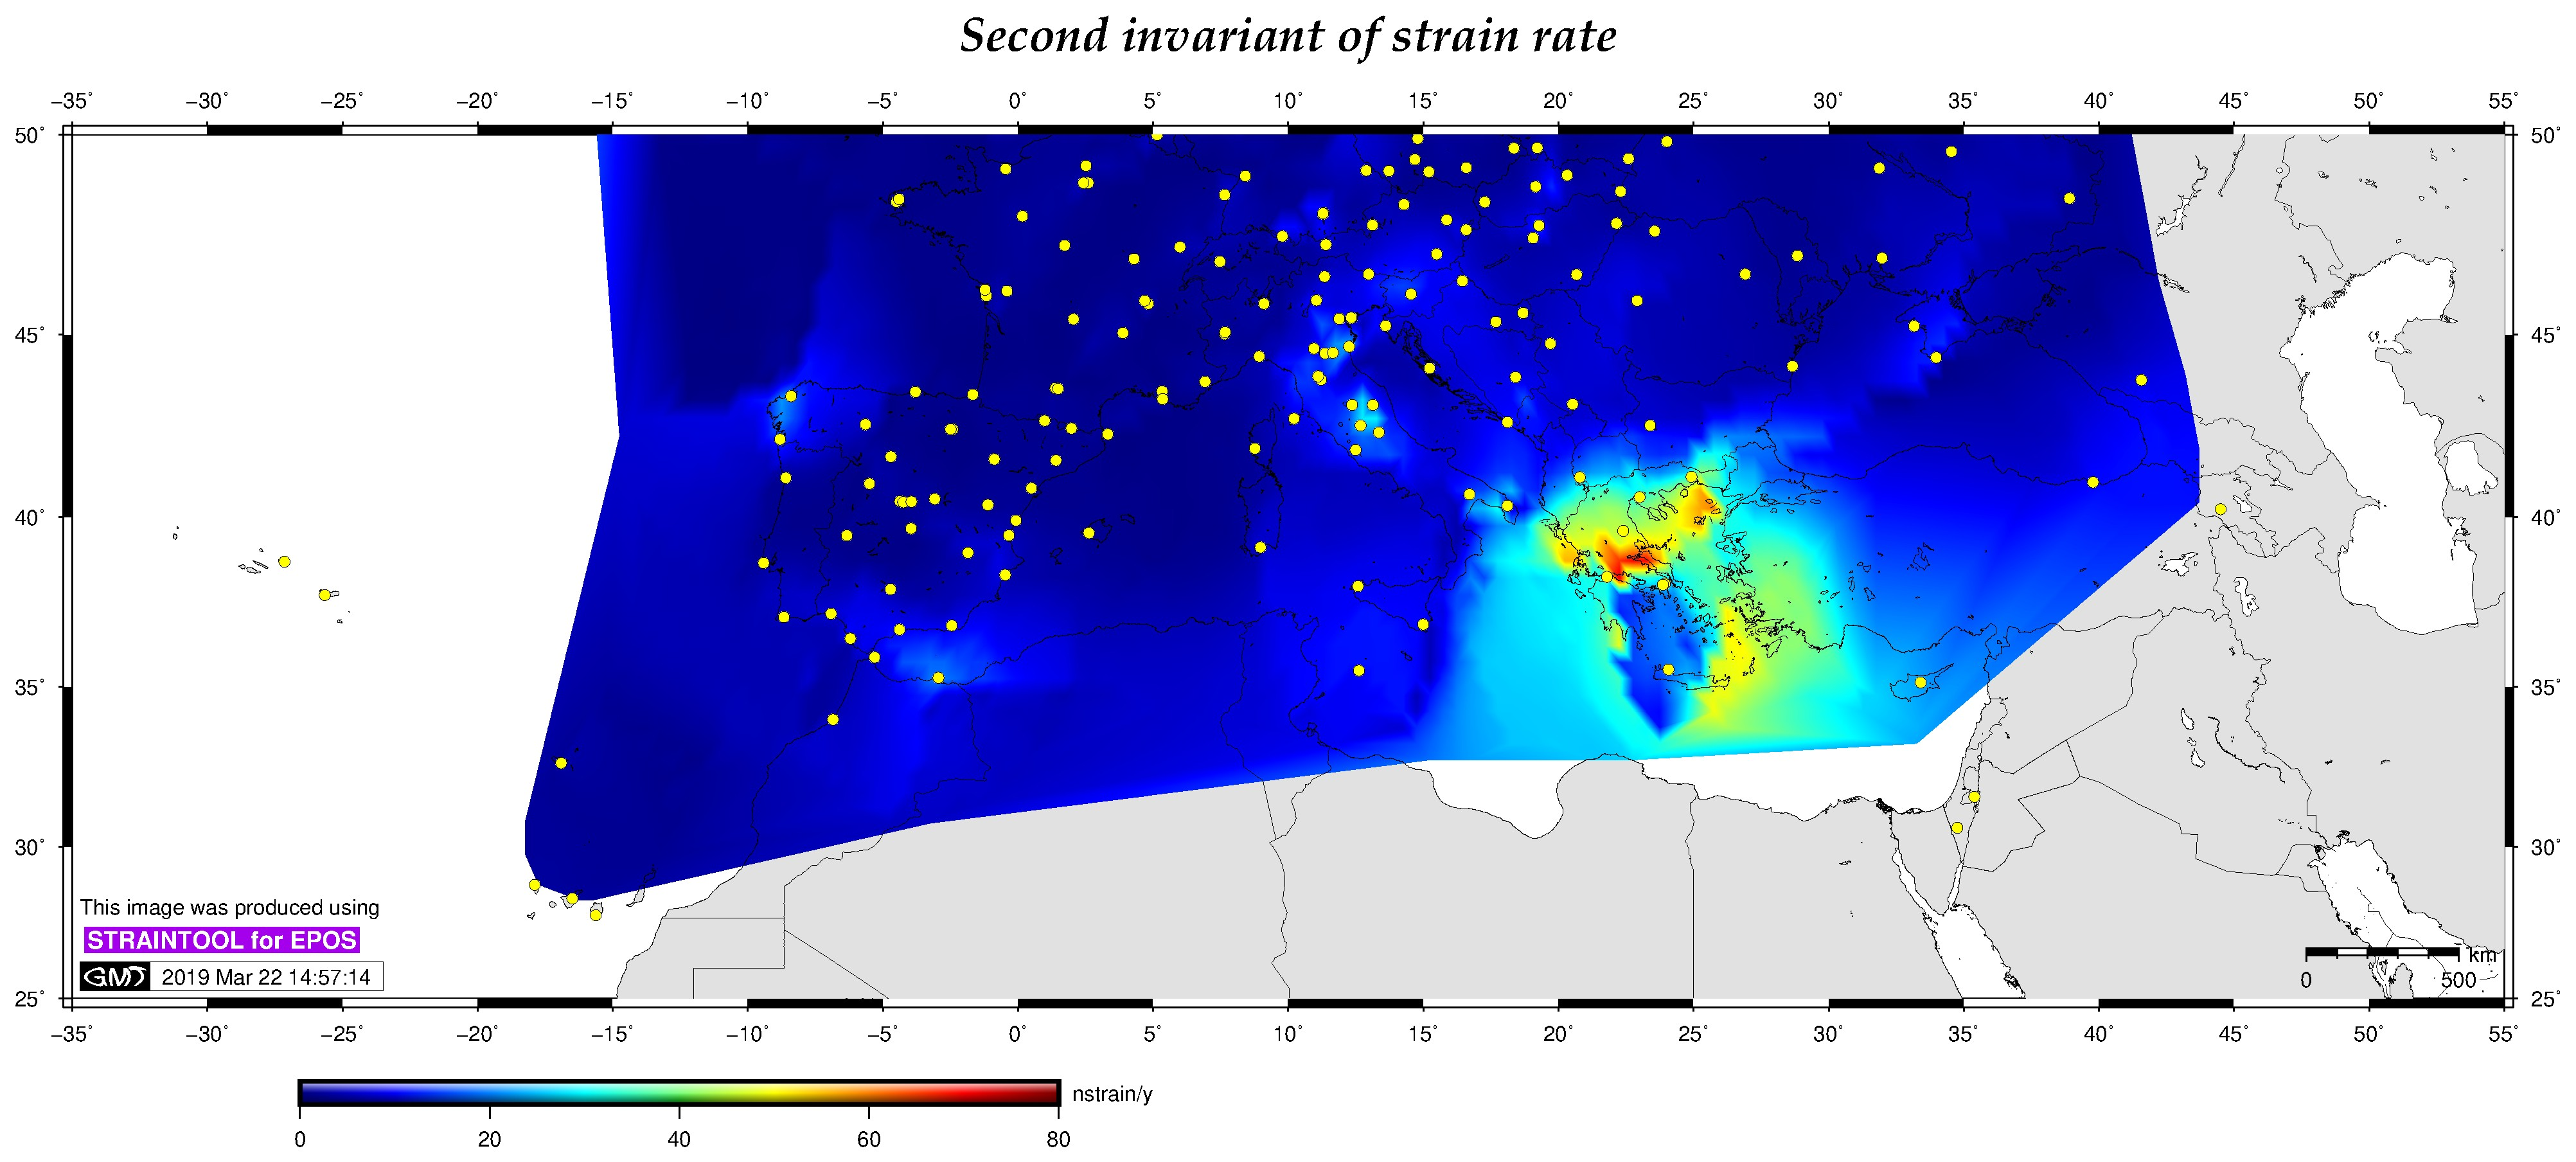
\includegraphics[width=\textwidth]{e14s050506-output_2inv-S.jpg}

% \end{minipage}

\end{minipage}\hfill
\begin{minipage}[b]{0.36\linewidth}
     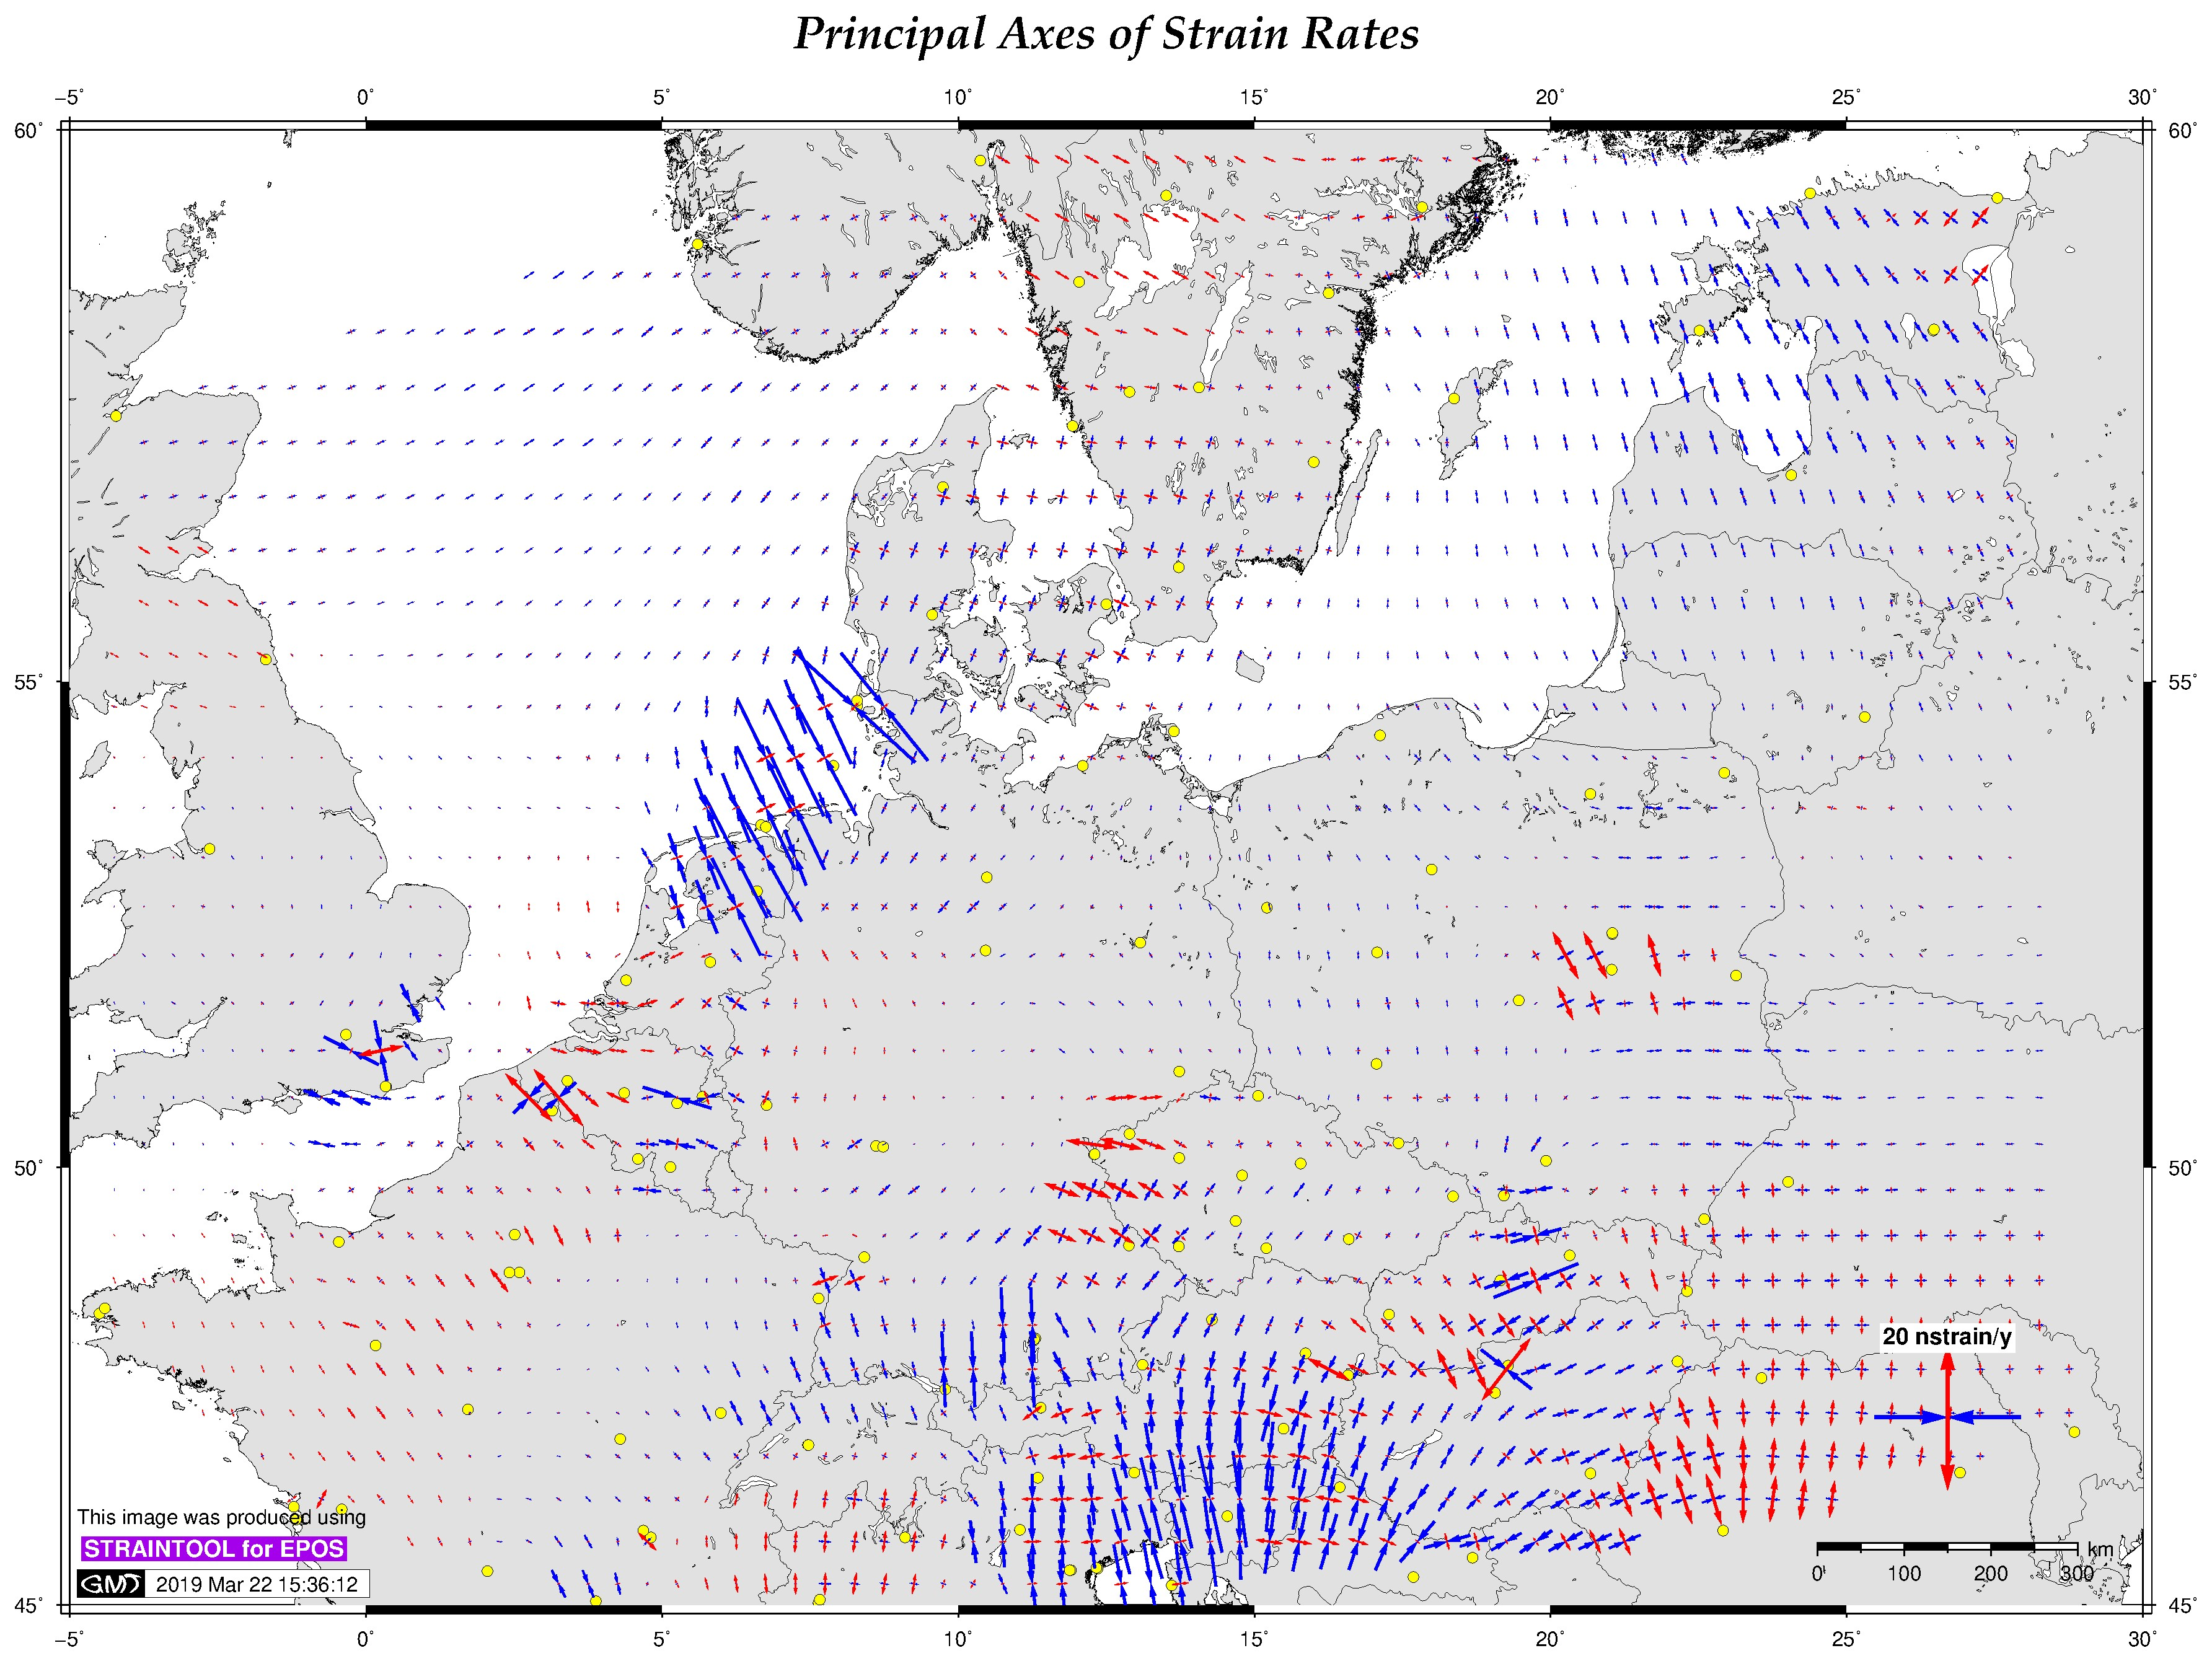
\includegraphics[width=.93\textwidth]{e14np050506e-output_str.jpg}
     
%      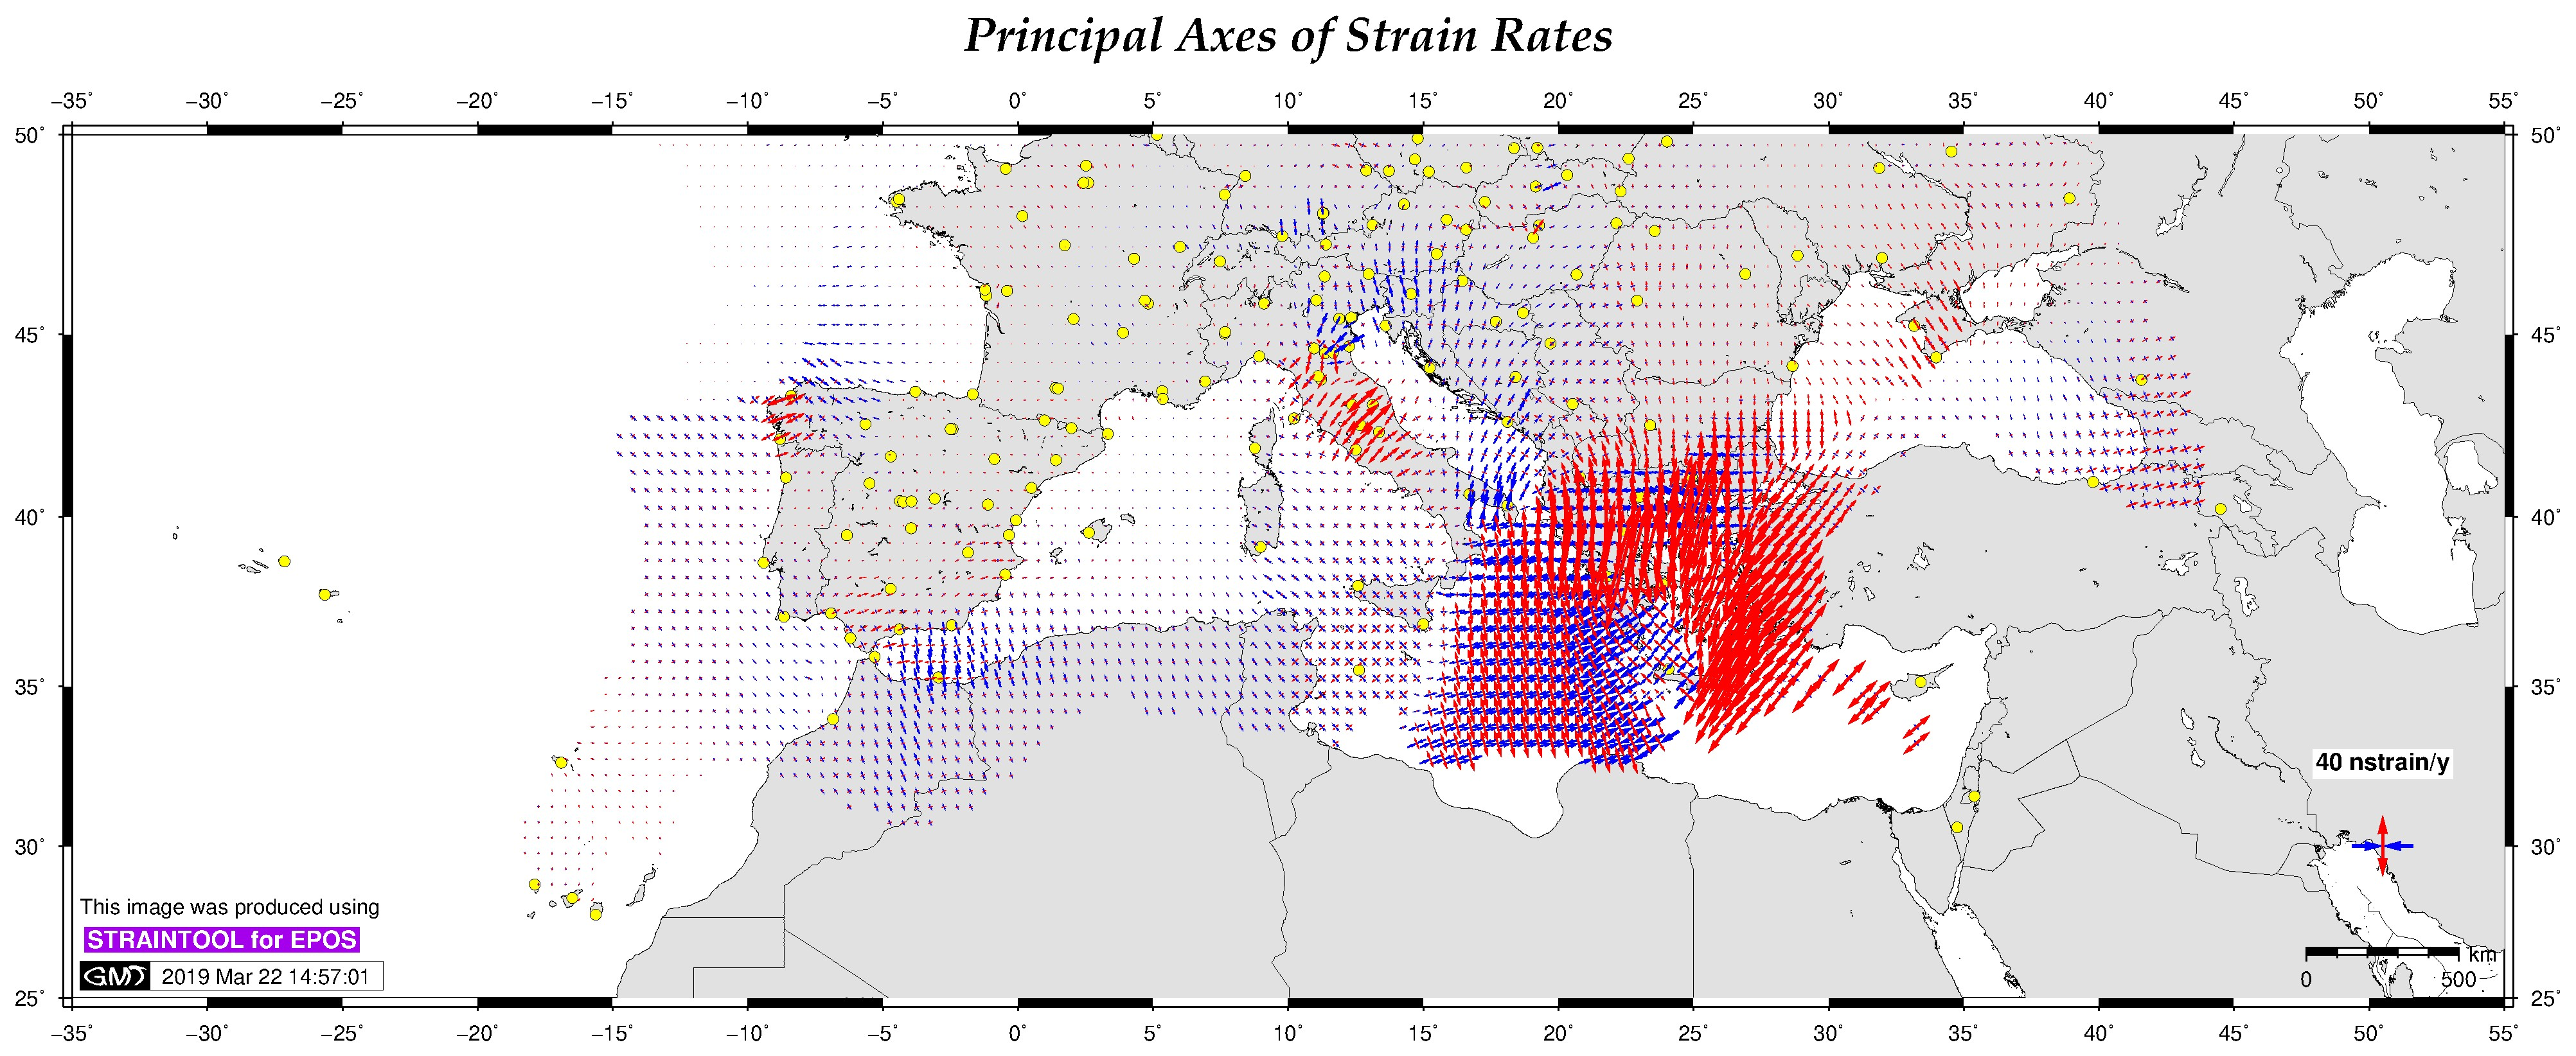
\includegraphics[width=\textwidth]{e14s050506-output_str-S.jpg}
     
     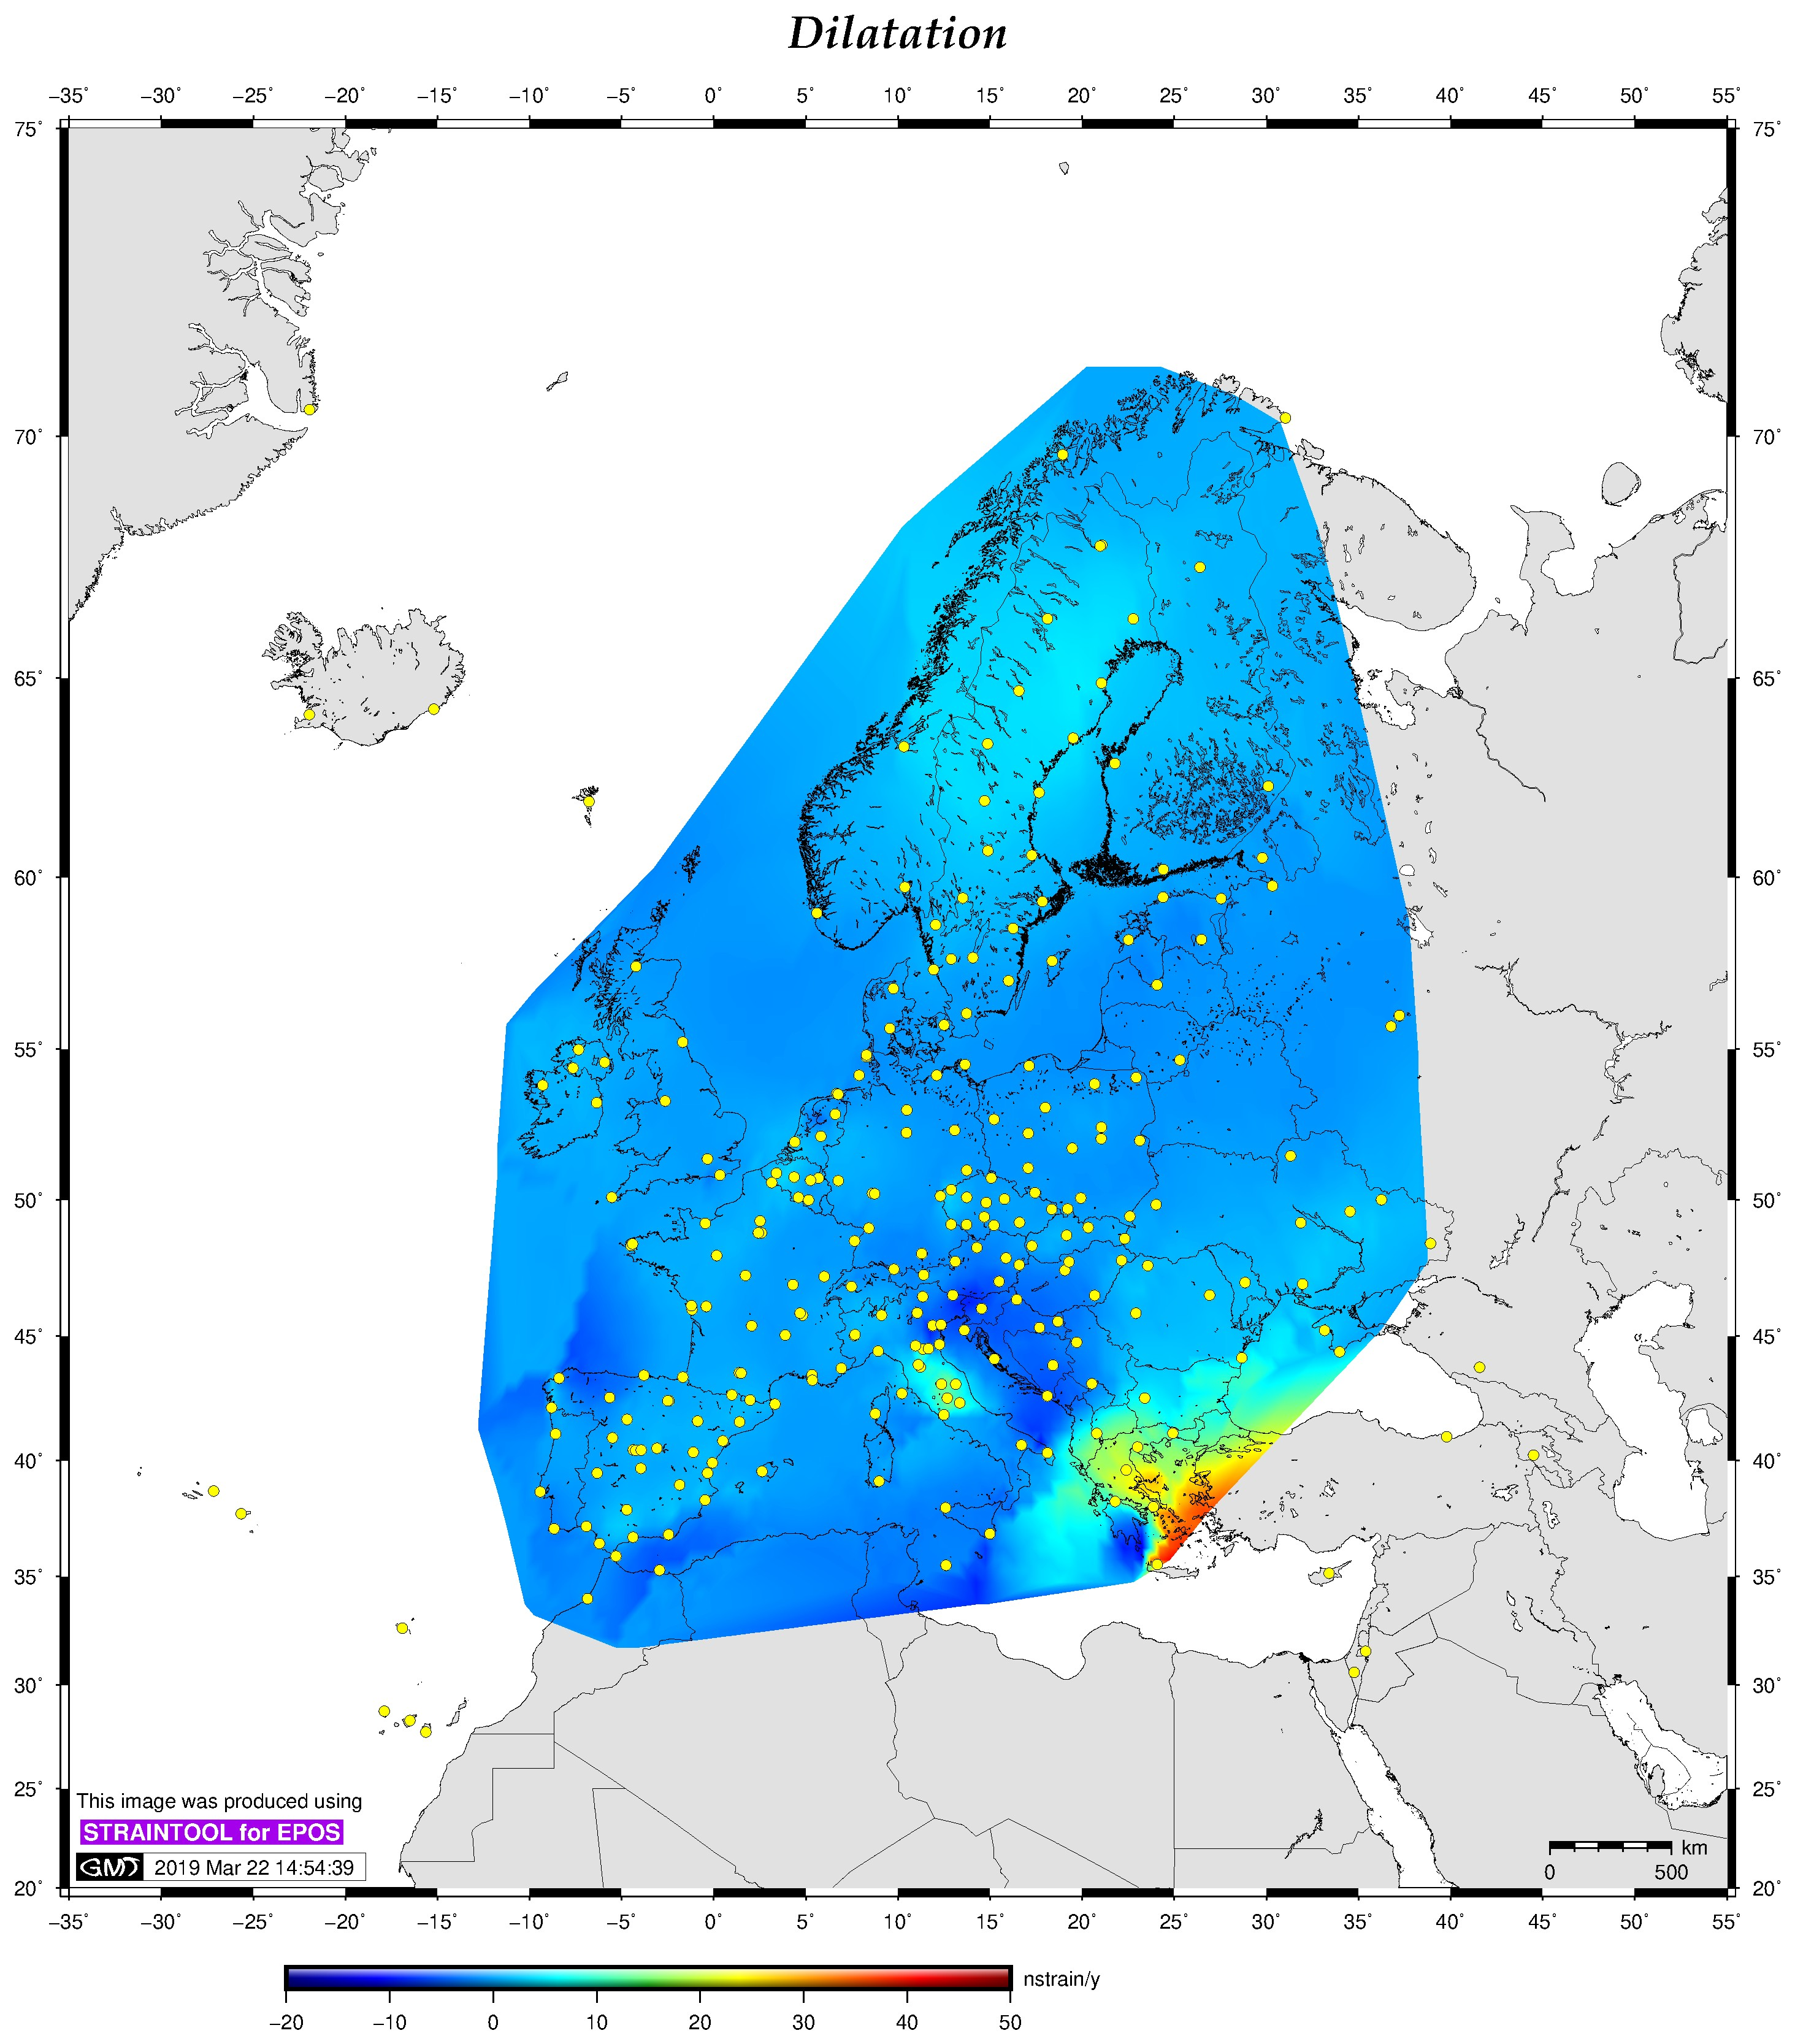
\includegraphics[width=.93\textwidth]{e14s050512-output_dil.jpg}
\end{minipage}

}

%----------------------------------------------------------------------------------------
%	STRAIN TOOL
%----------------------------------------------------------------------------------------

\headerbox{StrainTool}{name=straintool,column=0,below=introduction,bottomaligned=resval}{ 

\texttt{StrainTool} is a heighly customizable software package; users can configure the
estimation process using a list of input options. The basic input is a data file
containing station coordinates along with their respective volocity components.

Users can select the estimation of a single Strain Tensor (at the region's barycentre)
or estimation of multiple Strain Tensors placed on a (regular) grid within the 
region limits. Grid formation details are fully customizable by the user.

Estimation of the Strain Tensor parameters follows a Least Squares approach, based either
on \textbf{Veis et al., 1992} or \textbf{Shen et al., 2015}. In the latter case, a sophisticated weighting
scheme is used, controlled by the user via a list of command-line-options.

% \lipsum[2]
The estimated Strain Tensor parameters along with their corresponding \texttt{sigma}
values can be visualized with the distributed shell scripts \texttt{gmtstrainplot.sh} 
and \texttt{gmtstatsplot.sh}. Both programs use \texttt{GMT} (\textbf{Wessel et al., 2013}) to
plot results, drived by a user-defined configuration file.

}

%----------------------------------------------------------------------------------------
%	STRAIN ALGORITHMS
%----------------------------------------------------------------------------------------

\headerbox{algorithms}{name=algorithms,column=1,row=0,bottomaligned=resval}{ 

Given a set of stations (aka points on earth's surface) with their
corresponding east and north velocities, we can estimate (or compute)
strain tensor parameters, by solving for the system
\[
\begin{bmatrix}
  V_{x,S_1} \\ 
  V_{y,S_1} \\ 
  \cdots \\ 
  V_{x,S_n} \\ 
  V_{y,S_n} \\ 
\end{bmatrix}
=
\begin{bmatrix}
  1 & 0 & \Delta_{y_1}  & \Delta_{x_1} & \Delta_{y_1} & 0 \\
  0 & 1 & -\Delta_{x_1} &  0           & \Delta_{x_1} & \Delta_{y_1} \\
  \cdots & \cdots & \cdots & \cdots & \cdots & \cdots \\
  1 & 0 & \Delta_{y_n}  & \Delta_{x_n} & \Delta_{y_n} & 0 \\
  0 & 1 & -\Delta_{x_n} &  0           & \Delta_{x_n} & \Delta_{y_n} \\
\end{bmatrix}
\begin{bmatrix}
  U_{x} \\ 
  U_{y} \\ 
  \omega \\ 
  \tau_{x} \\ 
  \tau_{xy} \\ 
  \tau_{y} \\ 
\end{bmatrix}
\]
at any given location \(R\); \(\Delta_{x_i}\) and \(\Delta_{y_i}\) are the displacement
components between station \(i\) and the point \(R\). A minimum of 3 stations
is required to compute the parameters; if more than 3 stations are used, then
the parameters are estimated using a least squares approach.

\texttt{StrainTool} offers two approaches for computing strain tensors. A first, 
simple methodology is to split the region in Delaunay triangles, at the barycentre 
of which a strain tensor is computed. Note that this approach only uses three points 
to calculate tensor parameters, so the parameters are computed and not estimated.

A second more elaborate approach, uses covariance information and a sophistiacated
weighting scheme. A grid is constrcuted covering the study area and one strain 
tensor at the centre of each cell is estimated.
Assuming that we have variance information for the station velocities 
(and a Gaussian distribution), we can add the covariance matrix \(C\) of the 
velocity data in the system. In the simplest case, \(C\) is a diagonal matrix, 
with the velocity component standard deviations as its elements.

\textbf{Shen et al., 2015}, propose a more elaborate approach, reconstructing the
covariance matrix by multiplying a weighting function to each of its diagonal terms.
The weighting function is given by \(G_i = L_i \cdot Z_i\), in which \(L_i\) and \(Z_i\)
are functions of distance and spatial coverage dependent, respectively.
The final covariance matrix becomes then, \(C = C \cdot G^{-1}\) or, since its diagonal,
\(C_i = C_i \cdot {G_i}^{-1}\).
\(L_i\) is a distance-dependent weighting formula, in which a spatial smoothing 
parameter \(D\) is introduced and allows reduced weighting of the data as distance 
increases. It can have two forms, namely quadratic or Gaussian depending on the
spatial distribution of the data points. The the optimal smoothing parameter \(D\) 
is either selected by the user (and regarded constant) or searched for at each 
estimation.
The spatial weighting function \(Z_i\) measures the azimuth span of each site 
with respect to each of the remaining data points.

Both of the approaches, result in the computation or estimation of the parameter vector 
\([U_{x}, U_{y}, \omega, \tau_{x}, \tau_{xy}, \tau_{y}]^T\). In a second step, the
following quantities are computed and reported:
$$ \tau_{max}= \sqrt{ {\tau_{xy}}^2 + {e_{diff}}^2 } $$
$$ e_{max}  = e_{mean} + \tau_{max} $$
$$ e_{min}  = e_{mean} - \tau_{max} $$
$$ Az_{e_{max}}  = 90 + \frac{-atan2(\tau_{xy}, e_{diff})}{2} $$
$$ dilatation = \tau_{x} + \tau_{y} $$
$$ second invariant = \sqrt{ {\tau_{x}}^2 + {\tau_{y}}^2 + 2{\tau_{xy}}^2  }$$
where,
$$ e_{mean} = \frac{\tau_{x}+\tau_{y}}{2} $$
$$ e_{diff} = \frac{\tau_{x}-\tau_{y}}{2} $$
}

%----------------------------------------------------------------------------------------

\end{poster}

\end{document}
